\chapter{Design Considerations}
\vspace{-5 mm}
In this chapter the system is designed with a top-down approach, which means an overview of the system is formulated first. Thereafter the system will be broken down into smaller segments. First a use-case model of the system, where the functionalities and the coherent actors is described, in order to give an overview of what the system must be able to do. Thereafter, constraints set by time limitations as well as a focus on the main scope of the project, in regards to the prototype, are considered.
\vspace{-4 mm}
\section{Use case Design} \label{sec:UseCase}
To give an overview of what the system should be able to do, a use case with coherent actors is utilized. The use case diagram, see \figref{fig:usecase}, will describe the main functionalities in the use case as well as describing the actors, the external sensors and systems, affecting the system.

%The use-case diagram is made, where the micro controller is the system that will be analysed, because, it will be the master in this system

\vspace{-3 mm}
 \begin{figure}[H]
	\centering
	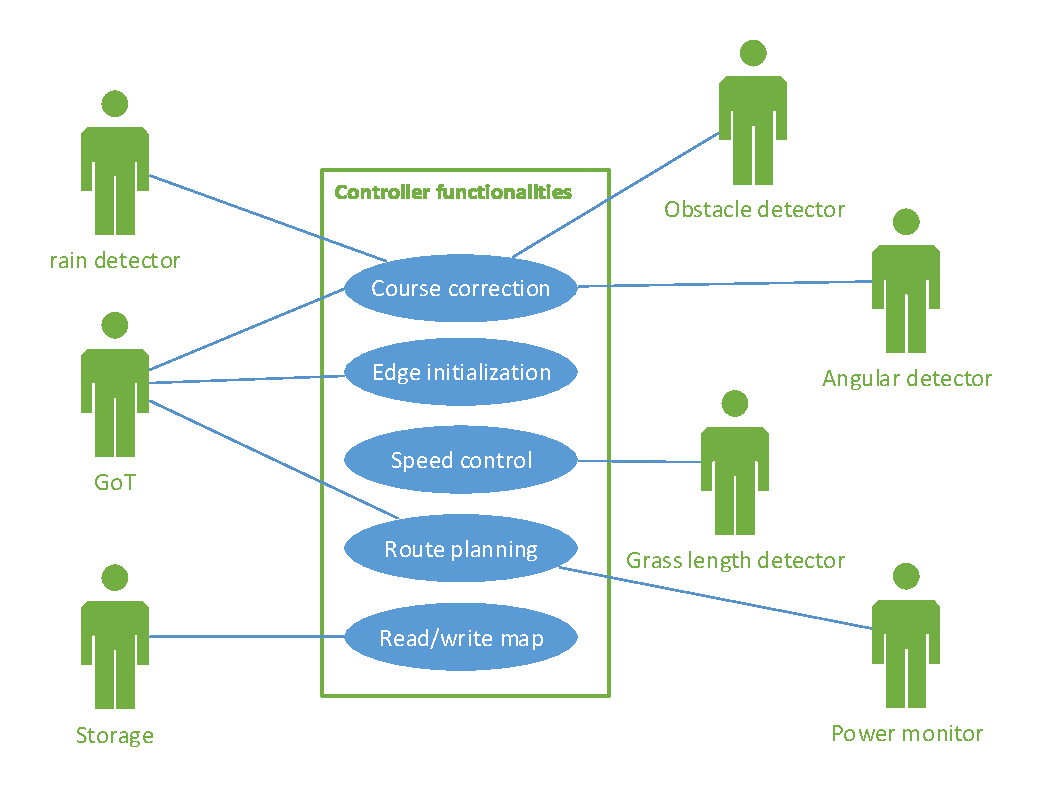
\includegraphics[scale=0.8]{figures/P5UseCase.pdf}
	\caption{Use-Case Diagram}
	\label{fig:usecase}
\end{figure}

\noindent
\newpage

The system, inside the controller, have 6 main functionalities and is affected by 9 different actors.

\subsection{Main Functionalities}

Functionalities are the functions that the system can do. Each Functionality can have more than one function in the system. The functionalities get input from actors and can be in association with other functionalities. 

\textbf{Edge Initialization}:
The \textit{Edge Initialization} gets input from the \textit{GoT} system and is associated with the \textit{Read/Write Map} functionality. The purpose of this function, is to calibrate the system to a new lawn. The function is making a edge map of the lawn. It used it to locate all the areas, where the lawn shall be mowed and where the lawn mower shall not drive. This is done, by manually moving the \textit{GoT} system's transmitter  along the edges of these areas. From the information about all the edges, the edge map is created and saved through the \textit{Read/Write Map} function.

\textbf{Route Planning}:
The \textit{Route Planning} gets input from the \textit{Power Monitor} and is associated with the \textit{Read/Write Map} functionality. The purpose of this function, is to plan the route for the lawn mower. The route is made from the information about where the lawn mower starts, the map of the lawn, which is made in the \textit{Edge Initialization} function. The map is loaded from the \textit{Storage} with the \textit{Read/Write Map} function. It also needs the battery level from the \textit{Power Monitor}. The route has to cover the whole lawn.

\textbf{Read/Write Map}:
The \textit{Read/Write Map} gets input from the \textit{Storage} and is associated with the \textit{Route Planning}, \textit{Course Correction} and the \textit{Edge Initialization} functionalities. This functionality communicates with the storage. In the \textit{Storage} the edge map from the \textit{Edge Initialization} function is saved and loaded from. The route from the \textit{Route Planning} is saved there to. The route is loaded and send to the \textit{Course Correction} functionality, when the system is driving.

\textbf{Course Correction}:
The \textit{Course Correction} gets input from the \textit{GoT} system, the \textit{Humidity Detector}, the \textit{Obstacle Detector} and the \textit{Angular Detector} and is associated with the \textit{Read/Write Map} and the \textit{Speed Control} functionalities. This function measures the surroundings of the lawn mower and makes corrections, in case of disturbances which might otherwise throw it off its route. The function makes the lawn mower stay on the route, which it get from the \textit{Read/Write Map} function, when the route can be followed. The \textit{Course Correction} is the main function behind the regulation of the movement of the lawn mower and sends these regulations to the \textit{Speed Control} function.

\textbf{Speed Control}:
The \textit{Speed Control} gets input from the \textit{Angular Detector}, the \textit{Grass Length Detector} and the \textit{Speed Measurement} and is associated with the \textit{Course Correction} functionality. The function's purpose, is to make sure that the lawn mower smoothly adapts the speed depending on the grass length, to get a more evenly cutting, and the curves of the route. This function controls the drive motor's speed, depending on route and regulation of the current speed.

\textbf{Blade Control}:
The \textit{Blade Control} gets input from the \textit{Blade Monitor}. The function's purpose, is keeping the blade rotational speed the same, to make an evenly cut. With the input from the \textit{Blade Monitor}, the \textit{Blade Control} regulate the speed to be constant.

\subsection{Actors}

A actor is a external system or component, that influence the system with inputs to the functionalities and/or gets output from them.

\textbf{Humidity Detector}:
The \textit{Humidity Detector} is connected to the functionality \textit{Course Correction}. This is a sensor that measures the humidity in the air. The system uses the information about the ambiant humidity level to see, whether it is too high to mow the lawn in or not, since wet grass can not be cut evenly and the cut of grass could damage the equipment. 

\textbf{GoT}:
The \textit{GoT} system is connected to the \textit{Course Correction} and \textit{Edge Initialization} functionalities. This system is used to get the lawn mower's position on the lawn. This position is sent to the controller, which uses the information to guide the lawn mower along its route.

\textbf{Storage}:
The \textit{Storage} is connected to the \textit{Read/Write Map} functionality. It uses a static storage to store the information about the edge map and route, which is made in the \textit{Edge Initialization} and \textit{Route Planning} functionalities. The \textit{Storage} will have the data saved, even if the system is turned off.

\textbf{Obstacle Detector}:
The \textit{Obstacle Detector} is connected to the \textit{Course Correction} functionality. This sensor detects, if there are any objects, which blocks the lawn mower's route. This sensor makes sure, that the lawn mower keeps a distance to any object, like a human or a dog that could interfere with its route.

\textbf{Angular Detector}:
The \textit{Angular Detector} is connected to the \textit{Course Correction} and \textit{Speed Control} functionalities. This sensor measures the angular position and movement of the lawn mower, whether it is intentional movement or if the lawn mower slips. This sensor is used as a feedback, to keep the lawn mower on the route.

\textbf{Grass Length Detector}:
The \textit{Grass Length Detector} is connected to the \textit{Speed Control} functionality. This sensor measure the  grass length, which affects the speed, at which the lawn mower should drive. If the grass is long and that it cuts, the lawn mower has to drive slower, to make sure that it doesn't get stuck in the grass and cut the grass evenly. 

\textbf{Power Monitor}:
The \textit{Power Monitor} is connected to the \textit{Route Planning} functionality. This sensor measures how much power  is left in the battery. This is needed, so that the lawn mower can drive back to its charging station, before the battery is empty.

\textbf{Blade Monitor}:
The \textit{Blade Monitor} is connected to the \textit{Blade Control} functionality. This sensor measures the rotational speed of the blade and send the information back to the \textit{Blade Control}, making a feedback loop.

\textbf{Speed Measurement}:
The \textit{Speed Measurement} is connected to the \textit{Speed Control} functionality. The sensor measure the speed, in which the lawn mower drive with. This information is send to the \textit{Speed Control} as feedback.